\documentclass[a4paper, titlepage]{article}
\usepackage[round, sort, numbers]{natbib}
\usepackage[utf8]{inputenc}
\usepackage{amsfonts, amsmath, amssymb, amsthm}
\usepackage{color}
\usepackage{listings}
\usepackage{mathtools}
\usepackage{paralist}
\usepackage{parskip}
\usepackage{subfig}
\usepackage{tikz}
\usepackage{titlesec}

% \numberwithin{figure}{section}
% \numberwithin{table}{section}

\usetikzlibrary{arrows, automata, backgrounds, petri, positioning}
\tikzstyle{place}=[circle, draw=blue!50, fill=blue!20, thick]
\tikzstyle{marking}=[circle, draw=blue!50, thick, align=center]
\tikzstyle{transition}=[rectangle, draw=black!50, fill=black!20, thick]

% define new commands for sets and tuple
\newcommand{\setof}[1]{\ensuremath{\left \{ #1 \right \}}}
\newcommand{\tuple}[1]{\ensuremath{\left \langle #1 \right \rangle }}
\newcommand{\card}[1]{\ensuremath{\left \vert #1 \right \vert }}

\makeatletter
\newcommand\objective[1]{\def\@objective{#1}}
\newcommand{\makecustomtitle}{%
	\begin{center}
		\huge\@title \\
		[1ex]\small Dimitri Racordon \\ \@date
	\end{center}
	\@objective
}
\makeatother

\begin{document}

\title{Outils formels de Modélisation \\ 6\textsuperscript{ème} séance d'exercices}
\author{Dimitri Racordon}
\date{27.10.17}
\objective{
  Dans cette séance d'exercices,
  nous allons étudier les graphes de couverture.
  Nous comparerons ces structure avec les graphes de marquage,
  et étudierons leurs relation avec les propriétés des réseaux de Petri.
}

\makecustomtitle

\section{Producteur/consommateur ($\bigstar\bigstar$)}

Considérez le réseau \emph{a} de la figure \ref{fig:producer-consumer},
lequel représente un modèle \emph{producteur consommateur}.

\begin{enumerate}
  \item Déterminez le rôle de chaque place et de chaque transition.
  \item Ce réseau est-il $k$-borné, et si oui pour quelle valeur de $k$?
  \item Déssinez le graphe de marquage et de couverture du réseau.
\end{enumerate}

\begin{figure}[ht]
	\centering
  \subfloat[]{%
    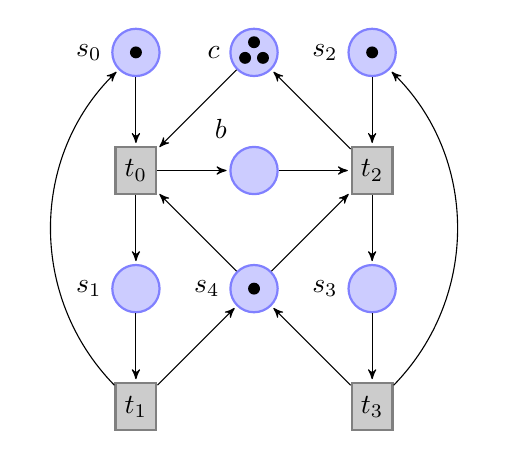
\begin{tikzpicture}[node distance=1.5cm, minimum height=6mm, >=stealth', bend angle=45, auto]
      \node[place,tokens=1] (s0) [label=left:$s_0$] {};
      \node[place]          (s1) [below of=s0, yshift=-1.5cm, label=left:$s_1$] {};

      \node[place,tokens=3] (cb) [right of=s0, label=left:$c$] {};
      \node[place]          (b)  [below of=cb, label=135:$b$] {};
      \node[place,tokens=1] (s4) [below of=b, label=left:$s_4$] {};

      \node[place,tokens=1] (s2) [right of=cb, label=left:$s_2$] {};
      \node[place]          (s3) [below of=s2, yshift=-1.5cm, label=left:$s_3$] {};

      \node [transition] (t0) [below of=s0] {$t_0$}
  				  edge [pre]  (s0)
            edge [pre]  (cb)
            edge [pre]  (s4)
            edge [post] (b)
            edge [post] (s1);
      \node [transition] (t1) [below of=s1] {$t_1$}
  				  edge [pre]  (s1)
            edge [post,bend left] (s0)
            edge [post] (s4);

      \node [transition] (t2) [below of=s2] {$t_2$}
  				  edge [pre]  (s2)
            edge [pre]  (s4)
            edge [pre]  (b)
            edge [post] (cb)
            edge [post] (s3);
      \node [transition] (t3) [below of=s3] {$t_3$}
  				  edge [pre]  (s3)
            edge [post,bend right] (s2)
            edge [post] (s4);
    \end{tikzpicture}
  }
  \subfloat[]{%
    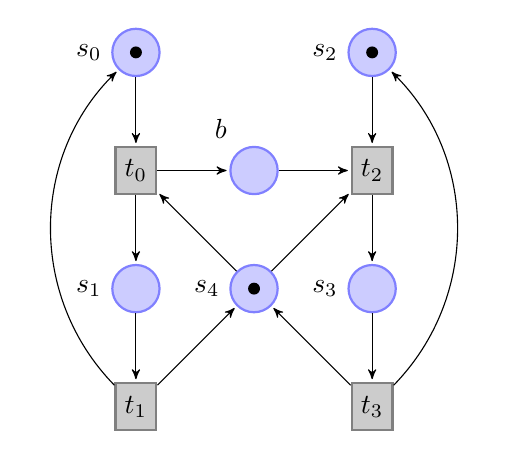
\begin{tikzpicture}[node distance=1.5cm, minimum height=6mm, >=stealth', bend angle=45, auto]
      \node[place,tokens=1] (s0) [label=left:$s_0$] {};
      \node[place]          (s1) [below of=s0, yshift=-1.5cm, label=left:$s_1$] {};

      \node                 (cb) [right of=s0] {};
      \node[place]          (b)  [below of=cb, label=135:$b$] {};
      \node[place,tokens=1] (s4) [below of=b, label=left:$s_4$] {};

      \node[place,tokens=1] (s2) [right of=cb, label=left:$s_2$] {};
      \node[place]          (s3) [below of=s2, yshift=-1.5cm, label=left:$s_3$] {};

      \node [transition] (t0) [below of=s0] {$t_0$}
        edge [pre]  (s0)
        edge [pre]  (s4)
        edge [post] (b)
        edge [post] (s1);
      \node [transition] (t1) [below of=s1] {$t_1$}
        edge [pre]  (s1)
        edge [post,bend left] (s0)
        edge [post] (s4);

      \node [transition] (t2) [below of=s2] {$t_2$}
  				  edge [pre]  (s2)
            edge [pre]  (s4)
            edge [pre]  (b)
            edge [post] (s3);
      \node [transition] (t3) [below of=s3] {$t_3$}
  				  edge [pre]  (s3)
            edge [post,bend right] (s2)
            edge [post] (s4);
    \end{tikzpicture}
  }
	\caption{Un modèle producteur/consommateur}
	\label{fig:producer-consumer}
\end{figure}

Considérez maintenant la variante \emph{b}.

\begin{enumerate}
  \item Ce réseau est-il $k$-borné, et si oui pour quelle valeur de $k$?
  \item Déssinez le graphe de marquage et de couverture du réseau.
\end{enumerate}

\section{Au chaud sous la converture ($\bigstar\bigstar$)}

Consédirez le graphe de couverture de la figure \ref{fig:couverture}.

\begin{enumerate}
  \item Déssinez un réseau de Petri dont le graphe de couverture serait le même.
  \item Combien d'autres réseaux pourraient avoir le même graphe de couverture?
  \item Le marquage $[1,0]$ est-il accessible?
  \item Le marquage $[0,2]$ est-il accessible?
  \item Ce graphe représente-t-il un réseau vivant?
\end{enumerate}

\begin{figure}[ht]
	\centering
  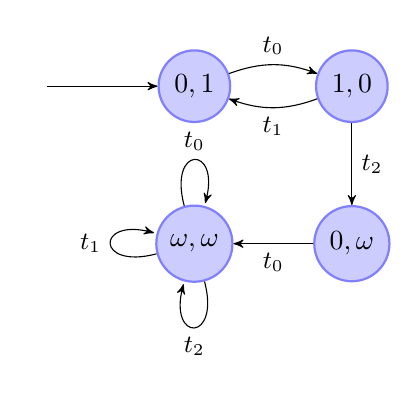
\begin{tikzpicture}[node distance=2cm, >=stealth', bend angle=20, auto]
    \node        (in)               {};
    \node[place] (n0) [right of=in] {$0, 1$};
    \node[place] (n1) [right of=n0] {$1, 0$};
    \node[place] (n2) [below of=n1] {$0, \omega$};
    \node[place] (n3) [left  of=n2] {$\omega, \omega$};

    \path[->, every node/.style={font=\sffamily\small}]
      (in) edge (n0)
      (n0) edge[bend left]  node [above] {$t_0$} (n1)
      (n1) edge[bend left]  node [below] {$t_1$} (n0)
      (n1) edge             node [right] {$t_2$} (n2)
      (n2) edge             node [below] {$t_0$} (n3)
      (n3) edge[loop above] node [above] {$t_0$} (n3)
      (n3) edge[loop left]  node [left]  {$t_1$} (n3)
      (n3) edge[loop below] node [below] {$t_2$} (n3);
  \end{tikzpicture}
	\caption{Graphe de couverture}
	\label{fig:couverture}
\end{figure}

\end{document}
